\section{Sentiments and Clusters}
We train a deep convolutional network on the Sentibank \cite{SentiBank} dataset, to classify images in a set of 2079 adjective-noun pairs, each of which have been assigned sentiments using crowd sourced effort. This network gave a top 5 match accuracy for the test dataset of 75\%. 
\par
The trained visual sentiment detector was then used on chronologically sampled frames from the vine videos collected. We sample 1 image per second for the 7 second long clips and hence now each video was being represented as a vector of 7 sentiment transition values. The main aim of this was to see if users are trying to tell stories in these short vine videos. One of the evidences of this would be clustering of similarly transitioning visual sentiments for videos across the dataset. 
\subsection{Choice of clusters}
The clusters were found using the basic k-means algorithm. For this to work we had to represent the videos in a vector representation. For this the videos were first passed through the deep convolutional network and the probability vector which was generated. These vectors were exhamined to  We used the elbow point method to find the right choice of clusters to find in our dataset. The metric we use to measure the tightness of clusters was average Minkowski's distance between cluster centroid and the data point vector. 
The Figure \ref{fig:elbow_points} shows the trend of average Minkowski from a cluster centroid as we increase the choice of cluster (k) from 1 to 10. The correct choice ofr k corresponds to the elbow points, or the points where the rate of decrease of average distance changes discontinually. We have 3 such prospective candidates at k = 3 , 4 and 5.
The grouping was found to be the tightest at k = 3 and k = 5.
Lets discuss what these choices actually mean in terms of sentiment transition values and their relevence to screenplay theories. 
\begin{figure}
\centering
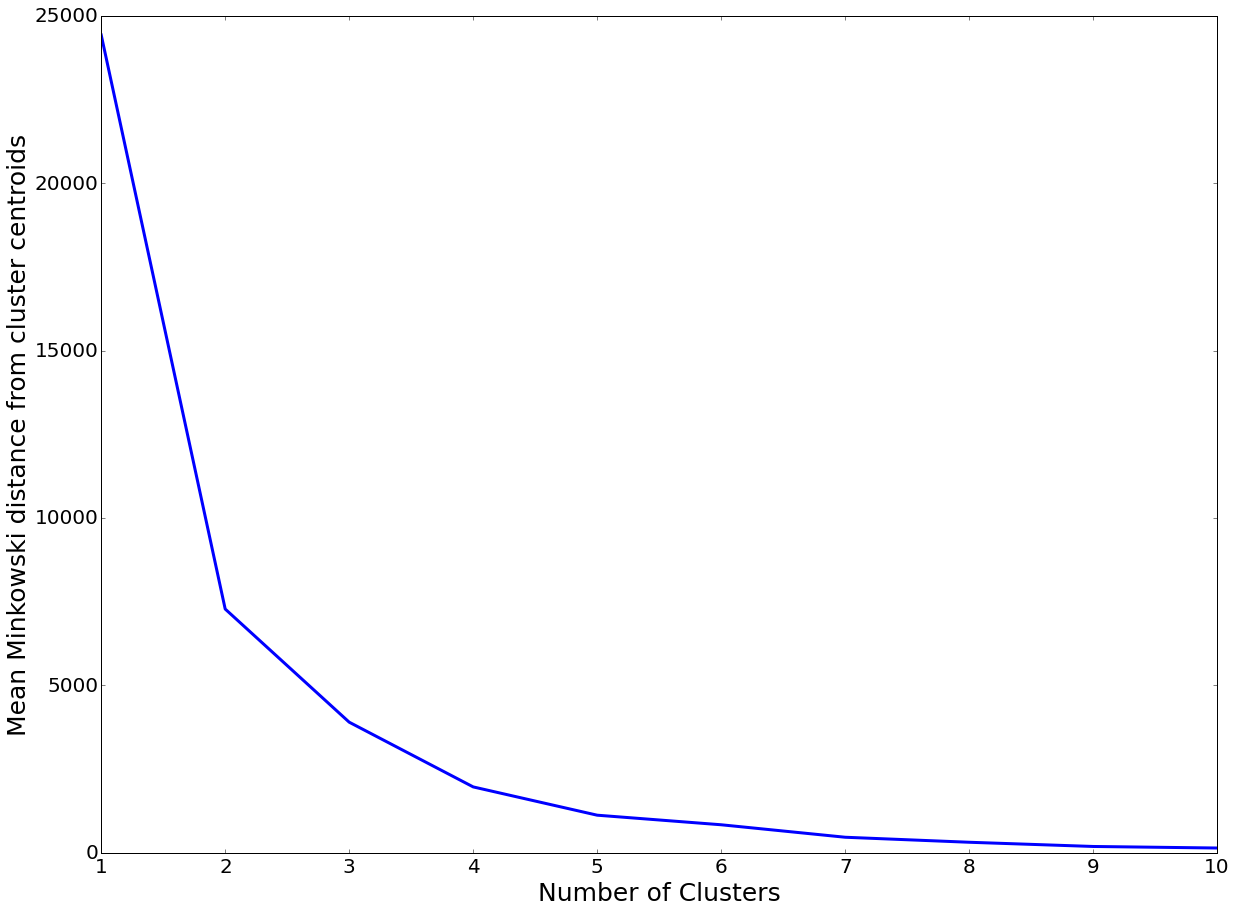
\includegraphics[width=\columnwidth]{plots/grouping_graph_clusters}
\caption{\textsl{This graph shows the variation of average minkowski distance of a sentiment vector from a cluster centroid for a given choice of K. The k is varied from 1 to 10.}}
\label{fig:elbow_points}
\end{figure}


\subsection{Clusters found}{
Let us look at the cluster choices individually. Figure \ref{fig:3_clusters}, \ref{fig:4_clusters} and \ref{fig:5_clusters} show these trends

\subsubsection{k=3}

For the choice of k=3, we see the most fundamental grouping of videos by visual perception. There are three distinct clusters with three kinds of perceptual sentiments. The first cluster is made up of all positive sentiments. Such videos mainly find adjective noun pairs which have adjectives like 'Cute' , 'Beautiful', 'Hot' , 'Handsome' et.al. These videos are mostly videos with protagonist being in the frame most of the time and is talking into the camera. This cluster is by sheer count has the biggest share of the pie. The second cluster is the cluster containing mostly negative perceptive sentiments. The adjectives that the network describes the frames by fall in the category of 'Sad' , 'Ugly' , 'messy' et.al.  The Third cluster has more of an oscillatory behaviour, where the first half of the video contains positive sentiments and the second negative. Figure \ref{fig:3_clusters} plots the centroids of the three clusters. Each curve on the plot represents the second by second sentiment value in the micro-video.
\par
The total number of videos belonging to first type are exactly twice to those belonging to the second type. This points towards a fact that users like to share fundamentally feel-good videos. 

\subsubsection{k=4}

For k=4, the grouping is weakest. But the signature of the two prime clusters of all negative and all positive sentiments still exist. The most populous two clusters are the all positive sentiments, followed by the all negative.  To explain the other two clusters, we have to move the the choice of k=5, where in the screenplay theories begin to correlate. 

\subsubsection{k=5}

This choice of k had the second best grouping amongst the 3 candidate choices. The two big clusters still follow the theme of mostly positive and mostly negative perceptive sentiments. But we see three interesting trends which follow three possible explaination based on the screenplay theories 
\par
We can first try analysing the sentiment trends using the popular Aristotle's three act play structure as discussed in Section \ref{Aristotle's Three Act Structure}. In this structure generally all stories can be fragmented into three segments. In each segment generally the story undergoes a turmoil or a drastic change in sentiment. In case of cluster C3, you can see these changes go towards a positive sentiment trajectory. 
}
\begin{figure}
\centering
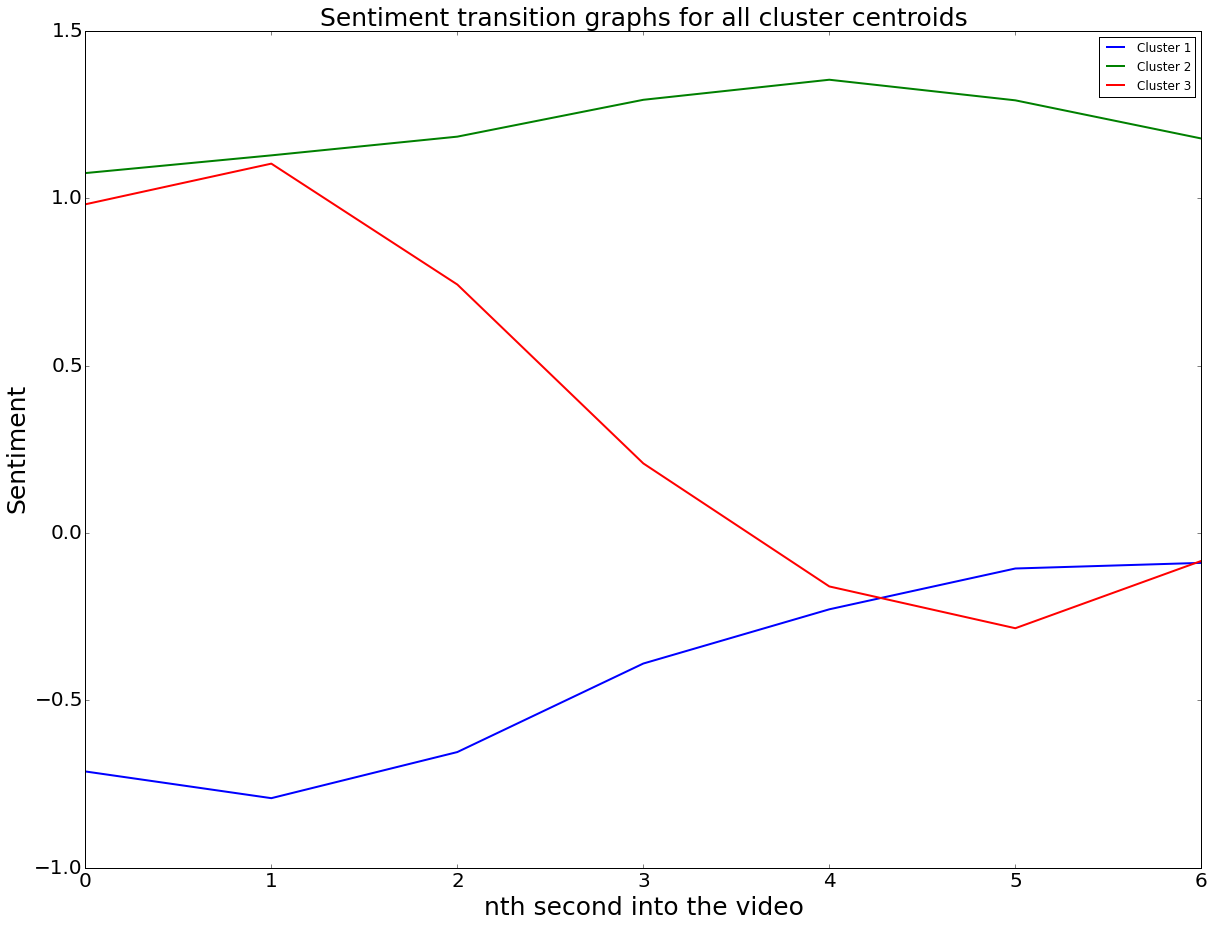
\includegraphics[width=\columnwidth]{plots/3_clusters_transitions}
\caption{\textsl{Sentiment values transitions for the centroids the clusters when K = 3.}}
\label{fig:3_clusters}
\end{figure}

\begin{figure}
\centering
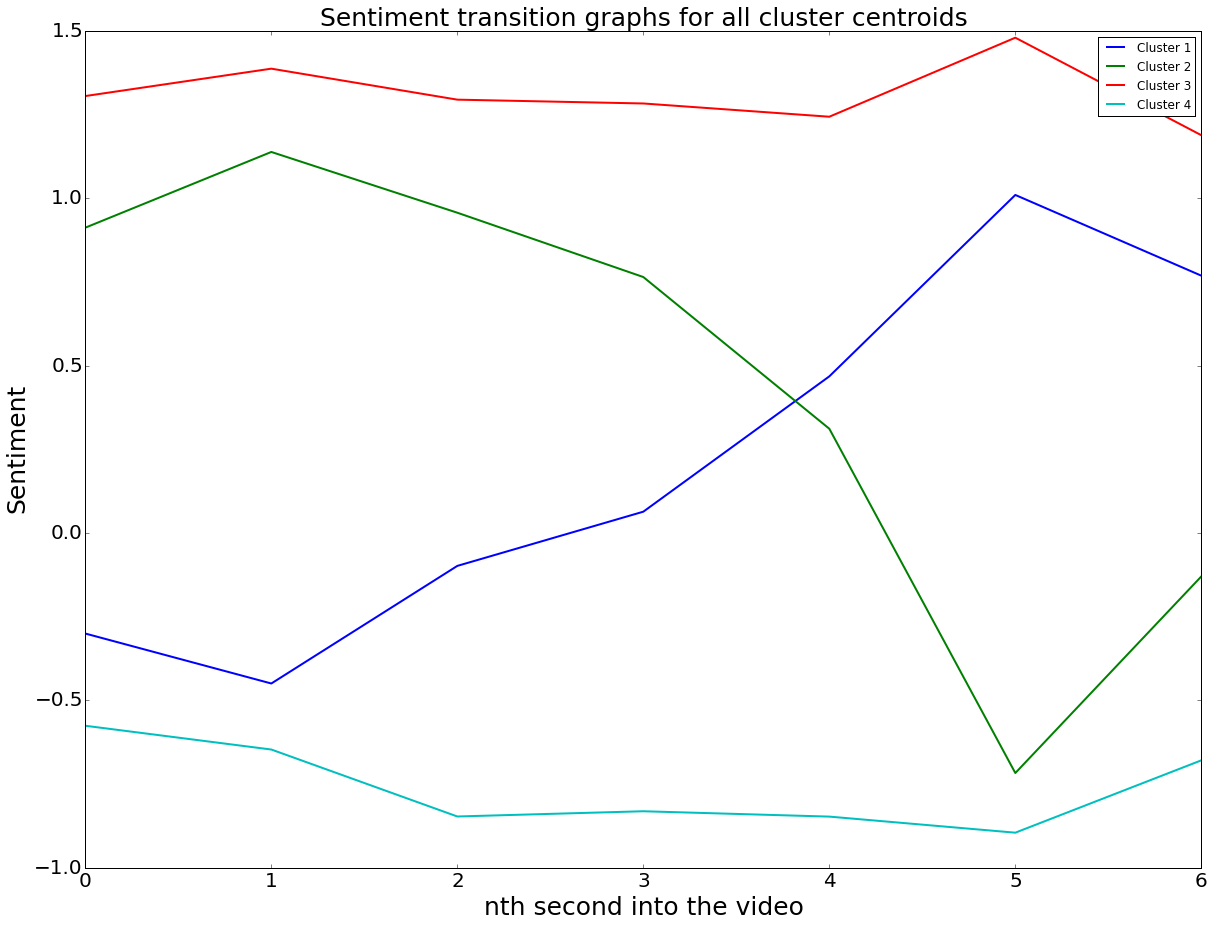
\includegraphics[width=\columnwidth]{plots/4_clusters_transitions}
\caption{\textsl{Sentiment values transitions for the centroids the clusters when K = 4.}}
\label{fig:4_clusters}
\end{figure}

\begin{figure}
\centering
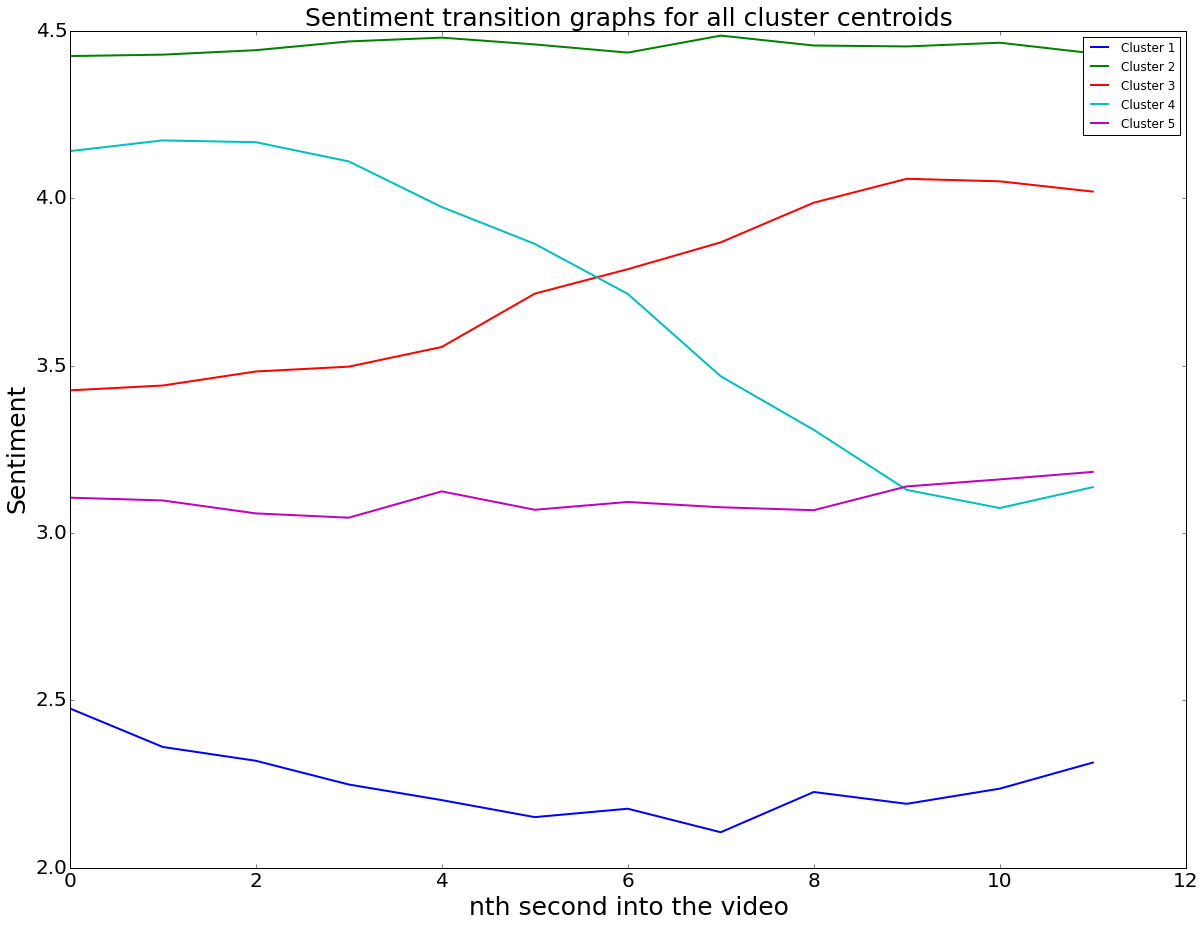
\includegraphics[width=\columnwidth]{plots/5_clusters_transitions}
\caption{\textsl{Sentiment values transitions for the centroids the clusters when K = 5.}}
\label{fig:5_clusters}
\end{figure}